% Overleaf 中文报告骨架（第 7 步模板）
% 使用方法见 README.md 第 6 节；编译引擎务必选 XeLaTeX（中文需要）
% ------------------------------------------------------------
\documentclass[11pt,a4paper]{ctexart}

% 页面与版式
\usepackage[margin=2.5cm]{geometry}
\usepackage{graphicx}
% 图片搜索路径：先找当前目录的 figures/，再找上一级目录的 figures/
% （main.tex 在 overleaf/ 里，figures/ 在项目根目录，所以用 ../figures/）
\graphicspath{{./figures/}{../figures/}}
\usepackage{booktabs}          % 三线表
\usepackage{amsmath}
\usepackage{hyperref}

% 图片默认居中
\setlength{\intextsep}{0.6cm}

\title{单座光伏电站 15 分钟级功率预测：\\基线对比与机器学习方法评估}
\author{【填姓名】\quad 【填学号】}
\date{\today}

\begin{document}
\maketitle

% ============================================================
\section{摘要}  % ---------- 你写 ----------
% 150~250 字。要点：研究问题、用了什么方法、主要数字结论、一句话指出局限/发现。
% 示例写法（照着这个骨架填，数字全部用你 results/ 里的真实值）：
%   本文以某光伏电站 2019 年全年 15 分钟粒度观测（35040 条）为对象，
%   对比 Persistence 基线、线性回归、随机森林与梯度提升树在两种信息设定下的预测性能。
%   结果表明：在可获得同时刻辐射的设定下，功率与总辐射 GHI 近似固定比例（斜率 0.1255），
%   线性公式的 MAE 为 0.0349 kW，优于随机森林（0.0378 kW）；
%   在只能使用历史观测的设定下，随机森林将 MAE 由 1.5374 kW 降至 0.6681 kW（降低 56.5\%）。
%   分场景分析进一步显示：模型价值集中在辐射剧烈变化时段（降幅 72.5\%），
%   而在辐射平稳时段反而劣于 Persistence 基线。
% ============================================================

% ============================================================
\section{引言}  % ---------- 你写 ----------
% 要写三件事：
%   (1) 背景：光伏并网调度为什么需要功率预测；
%   (2) 前人做到哪：对应 参考文献候选清单 里选的 1 篇综述 + 1 篇方法论文；
%   (3) 你的研究问题 + 本文结构（就是第 2 节那两个问题）。
%
% 引用示例（.bib 里有就写 \cite{antonanzas2016}）：
%   光伏功率预测可分为间接法与直接法两大类\cite{antonanzas2016}，
%   其中随机森林等集成学习方法在超短期预测中表现良好\cite{yang2021}。

% ============================================================
\section{数据与方法}
% ------------------------------------------------------------
\subsection{数据说明}
% 数据来源（站点 + 机构 + 链接）、时间范围、粒度、行数列数。已向数据提供方核实。
本实验采用宁夏光伏电站 2019 年全年、15 分钟粒度的发电与气象观测数据，
共 35040 条记录、20 个变量，时间自 2019-01-01 00:15 至 2019-12-31 23:45
（含首条至 2020-01-01 00:00 的采样结束时刻）。
数据由 Science Data Bank 公开发布（版本 V1，2025 年 5 月 29 日在线发布）\cite{ningxia2019photovoltaic}，
DOI 为 10.57760/sciencedb.25490。
主要变量包括：太阳总水平辐射 GHI、直接辐射 DNI、散射辐射 DHI、固定倾角斜面辐射 GTI、
气温、云层不透明度、相对湿度、10\,m 风速、风向、地面气压、露点温度、大气可降水量、
降雪深度，以及本文的预测目标——电站交流输出功率（实际功率，单位 kW）。

需要说明的是，该数据集页面未公开电站经纬度、海拔与装机容量，
故本文仅报告观测统计量（观测时段内最大瞬时功率 128.0403\,kW），不对上述元数据进行推测。

% ------------------------------------------------------------
\subsection{数据质量检查}  % ---------- 你写 ----------
% 填这几条真实结论：
%   · 35040 行 × 20 列，时间 2019-01-01 00:15 ~ 2020-01-01 00:00，间隔 15 分钟；
%   · 20 列零缺失；时间戳无重复、严格递增；35040 = 365 × 96，全年无缺口；
%   · 目标列 49.1\% 为 0（夜间不发电，属正常现象，不作为缺失值处理）；
%   · 以总辐射为判据做物理一致性检查，真正违反物理的异常样本为 0 条。

% ------------------------------------------------------------
\subsection{实验设定与评估指标}
% 写清楚这两个设定（这是你报告的方法核心，答辩必问）：
%   设定甲：同时刻气象；
%   设定乙：仅用历史观测（1/2/3…刻钟前的辐射与功率）。
% 再写：前 70\% 训练 / 后 30\% 测试，按时间先后切分、不打乱（防数据泄露）；
% 指标 MAE / RMSE / R²；随机种子 random\_state=42。

% ============================================================
\section{结果与分析}  % ---------- 你写 ----------
% ------------------------------------------------------------
\subsection{总体预测性能}
% 把你 results/metrics_step4.csv 的表搬过来（表 1）。
\begin{table}[htbp]
\centering
\caption{两种设定下的预测误差对比}
\label{tab:metrics}
\begin{tabular}{lccc}
\toprule
设定 \& 方法 & MAE (kW) & RMSE (kW) & $R^2$ \\
\midrule
%\ 甲 基线 & 0.0349 & 0.0737 & 1.0000 \\
%\ 甲 线性回归 & 0.0362 & 0.0738 & 1.0000 \\
%\ 甲 随机森林 & 0.0378 & 0.0827 & 1.0000 \\
%\ 甲 GBDT & 0.0953 & 0.1879 & 0.9999 \\
%\ 乙 基线 & 1.5374 & 2.7803 & 0.9888 \\
%\ 乙 线性回归 & 0.9397 & 1.6682 & 0.9960 \\
%\ 乙 随机森林 & 0.6681 & 1.5715 & 0.9964 \\
%\ 乙 GBDT & 0.7627 & 1.6016 & 0.9963 \\
\bottomrule
\end{tabular}
\end{table}
% ↑ 上面 8 行就是删掉 \% 号后的真实数字，你照抄进来（ kilowatt 记 2 位小数即可 ）

\begin{figure}[htbp]
\centering
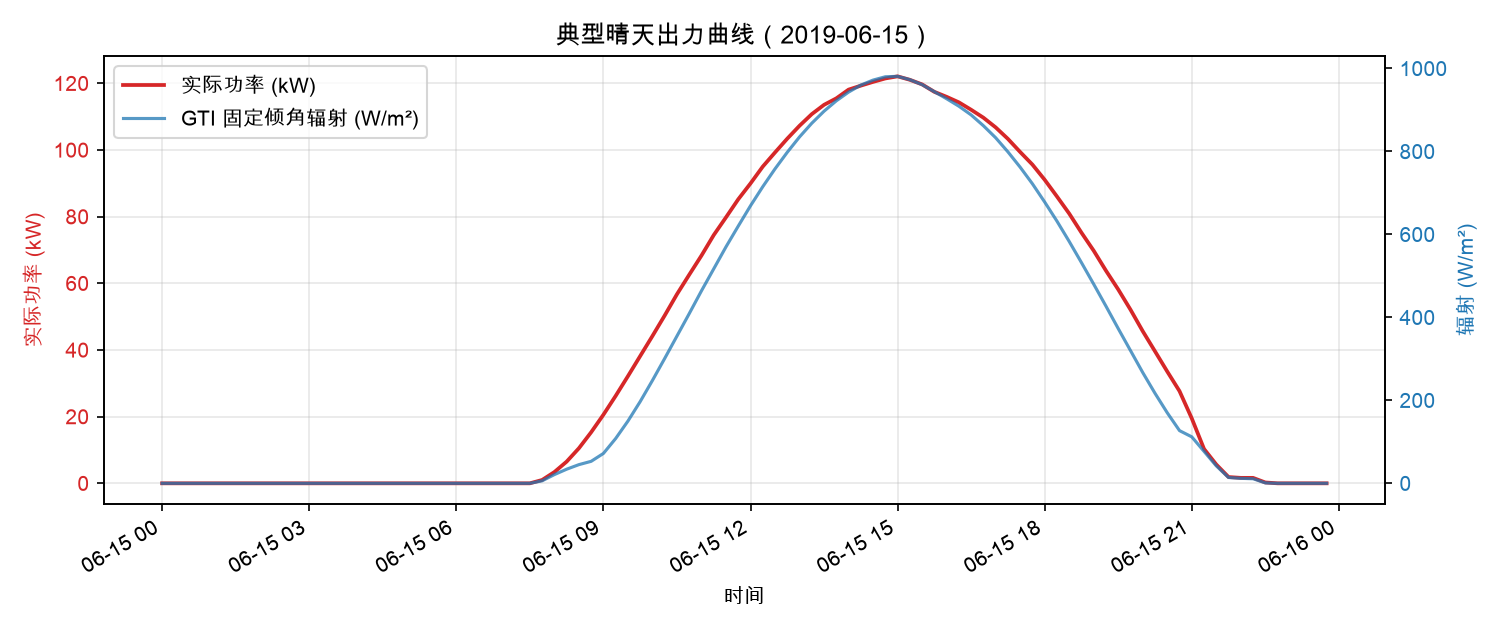
\includegraphics[width=0.9\textwidth]{fig1_typical_day}
\caption{典型日发电功率与辐射的时间序列}
\label{fig:typical}
\end{figure}

% ------------------------------------------------------------
\subsection{误差的天气分布（拓展①）}
% 把 metrics_step5_weather.csv 的「按辐射突变」那张表搬过来，配图 5。
\begin{figure}[htbp]
\centering
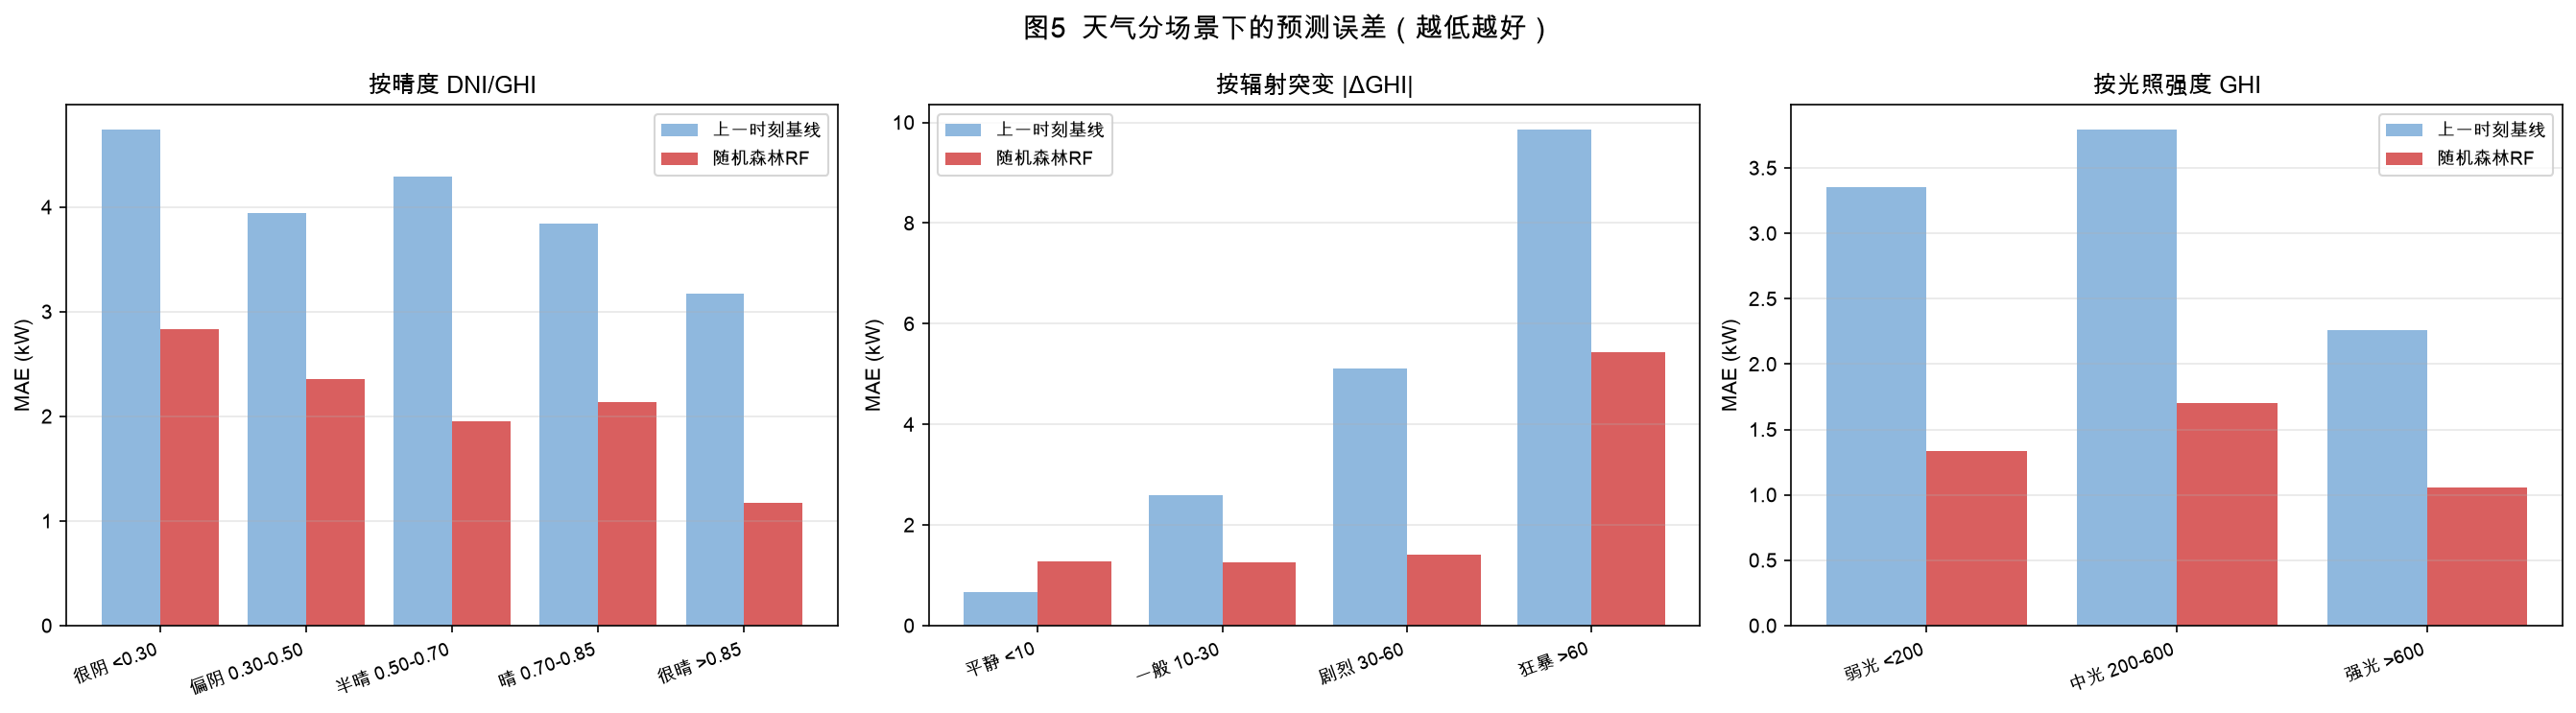
\includegraphics[width=0.95\textwidth]{fig5_weather_scenarios}
\caption{不同天气场景下的模型误差}
\label{fig:weather}
\end{figure}
% 结论一句话：模型价值集中在辐射剧烈变化时段；辐射平稳时 Persistence 已足够。

% ------------------------------------------------------------
\subsection{特征重要性（拓展②）}
\begin{figure}[htbp]
\centering
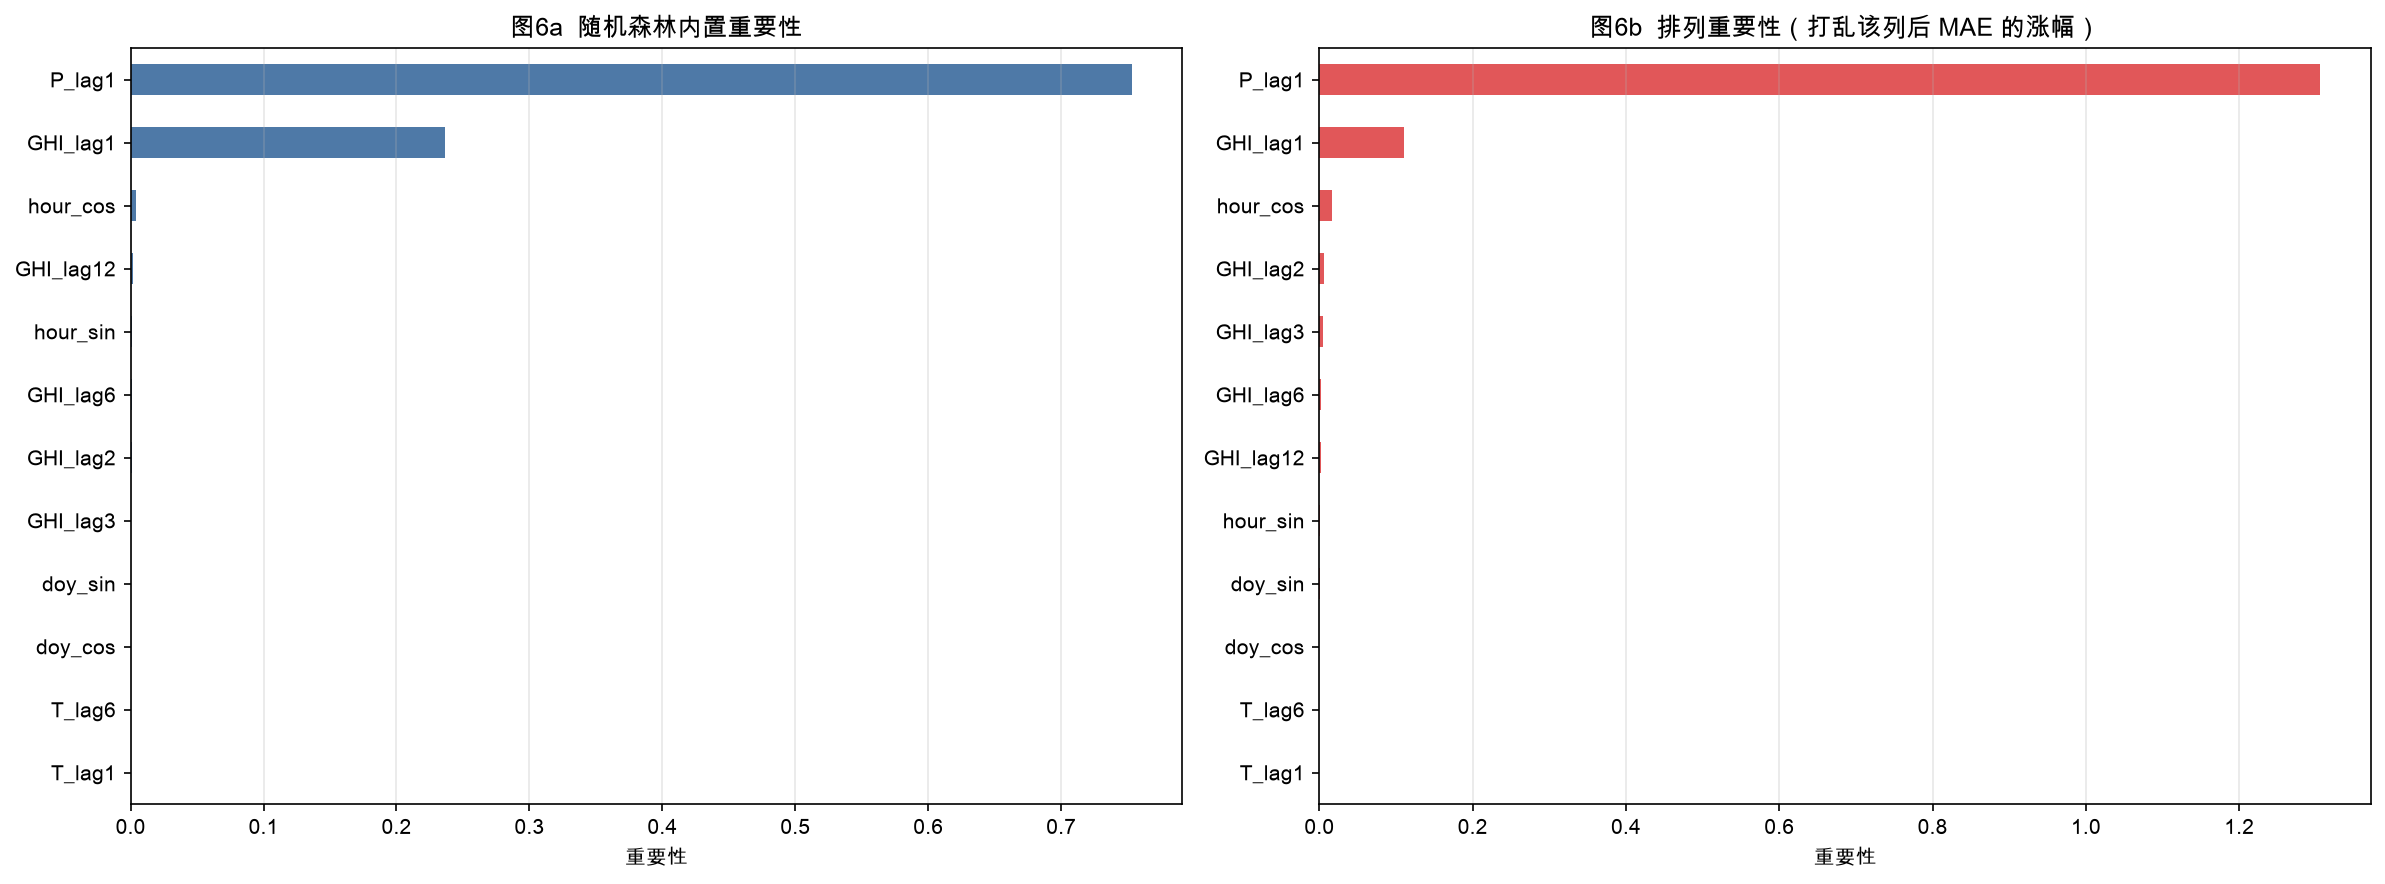
\includegraphics[width=0.9\textwidth]{fig6_feature_importance}
\caption{特征重要性与排列重要性}
\label{fig:importance}
\end{figure}
% 结论：P\_lag1 占绝对主导；气温两列重要性约等于 0。

% ------------------------------------------------------------
\subsection{温度与云量对预测的影响（补充实验）}  % ---------- 你写 ----------
% 数据提供方建议"预测时不考虑温度和云量"。为验证该经验判断，做了三问。
% 真实数字见 code/05_feature_ablation.py 与 results/metrics_step6_*.csv。

% 问1：白天（GHI>50 W/m²）样本 14854 条，功率与各因子的 Pearson 相关系数
%      GHI 1.0000 ｜ 云层不透明度 -0.5327 ｜ 相对湿度 -0.3954 ｜ 气温 +0.3878 ｜ 风速 +0.0338
%
% 问2：控制变量。把 GHI 每 50 W/m² 划为一档、只看档内样本（档内辐射基本一致），
%      拟合「功率~温度」斜率，各档平均 +0.0080 kW/℃，绝对值最大 0.0376 kW/℃；
%      而对照量 GHI 每增加 100 W/m²，功率约增加 12~13 kW。
%      → 温度效应比辐射效应小 1~2 个数量级。
%      注意：光伏组件温度每升 1℃ 功率本应约降 0.3\%~0.4\%
%      （满发 128 kW 时约 -0.45 kW/℃），本文实测却得到 +0.0080 kW/℃（符号甚至为正）。
%      原因是本站气温与晴天高辐射高度共线，温度效应被辐射效应掩盖。此处务必如实写出。

% 问3：消融实验（随机森林，同一时间切分）
\begin{table}[htbp]
\centering
\caption{特征消融实验结果（随机森林）}
\label{tab:ablation}
\begin{tabular}{lcc}
\toprule
特征集 & 特征数 & MAE (kW) \\
\midrule
甲 完整（含温度+云量） & 12 & 0.0378 \\
甲 只删温度 & 11 & 0.0379 \\
甲 只删云量 & 11 & 0.0378 \\
甲 温度云量都删 & 10 & 0.0379 \\
乙 完整（含温度滞后） & 8 & 0.8093 \\
乙 删掉温度滞后 & 6 & 0.8352 \\
\bottomrule
\end{tabular}
\end{table}
%
\begin{figure}[htbp]
\centering
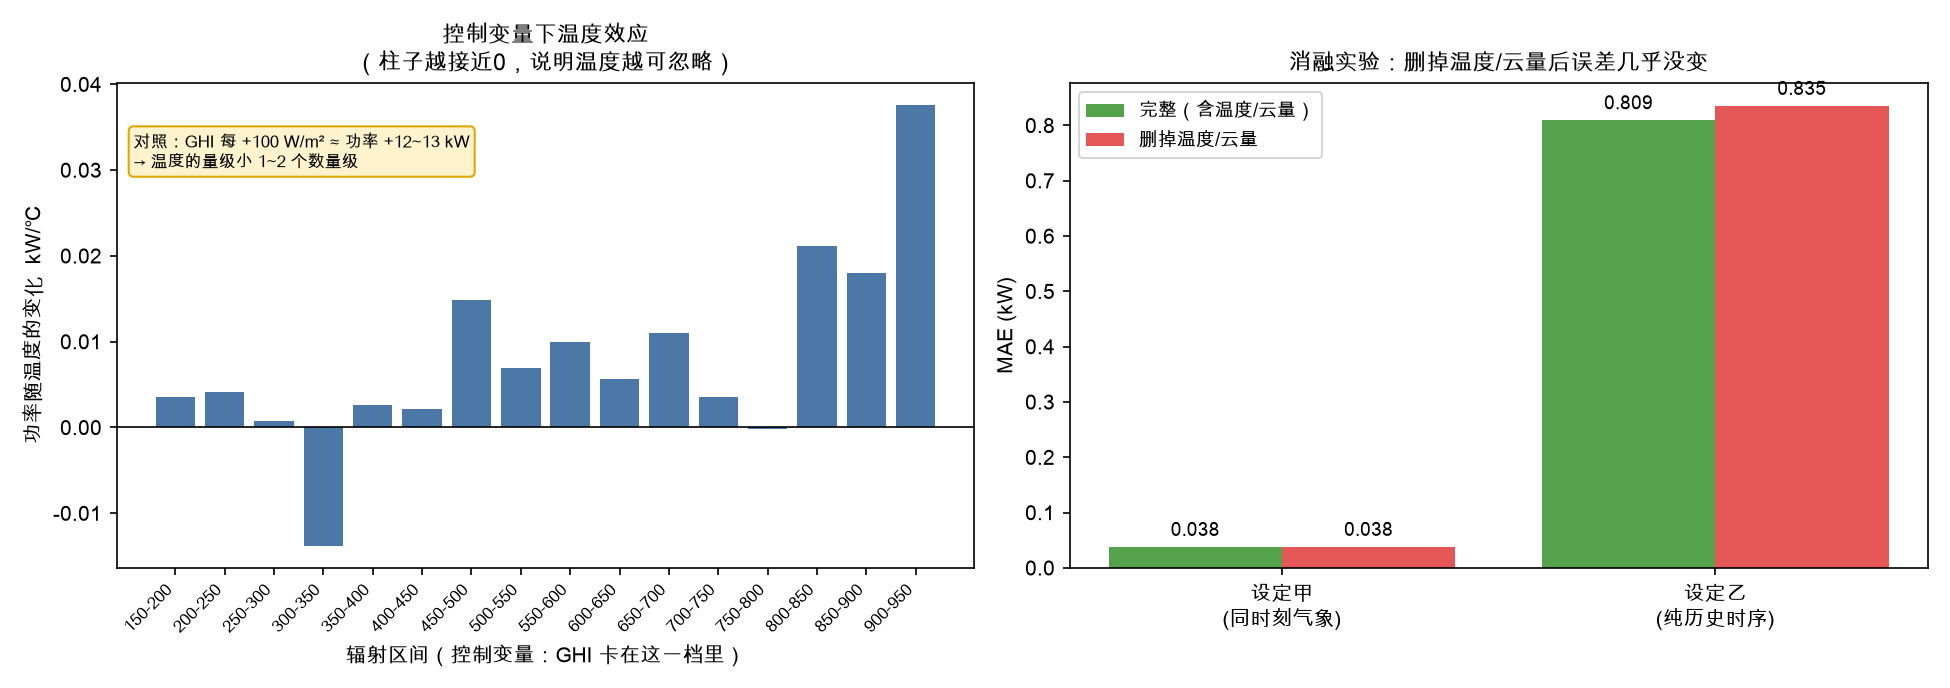
\includegraphics[width=0.9\textwidth]{fig7_ablation_temp_cloud}
\caption{控制变量下的温度效应（左）与特征消融的 MAE 对比（右）}
\label{fig:ablation}
\end{figure}
%
% 结论（这段话建议背下来，答辩必问）：
%   (1) 数据提供方的经验判断在本数据集上成立：删去温度与云量后 MAE 仅上升
%       0.26\%（设定甲）至 3.20\%（设定乙），可认为贡献可忽略；
%   (2) 但正确表述不是"温度对光伏没有物理影响"。温度效应真实存在，
%       只是在本站数据中被辐射效应掩盖（共线），模型的边际增益小于 3\%；
%   (3) 云层不透明度相关系数达 -0.53 却几乎无独立贡献，说明它与辐射高度共线，
%       模型用 GHI 即可"补上"其信息（特征冗余）。

% ------------------------------------------------------------
\subsection{关于目标列性质的检验}  % ---------- 你写 ----------
% 这一段是加分段落，如实写你查到的三件事：
%   (1) 功率与 GHI 近似固定比例（斜率 ≈ 0.125498，比值变异系数 CV ≈ 0.23\%）；
%   (2) 该比例与气温、云量的相关性接近 0，温度效应被抹平；
%   (3) 排列重要性中气温两列 ≈ 0。
% 并写明：站名与数据来源已确认（见数据说明），但"该列是否为实测计量值"
% 尚未获得数据提供方的书面确认，本文全程如实报告这一发现、不下结论。

% ============================================================
\section{结论}  % ---------- 你写 ----------
% 三小段：主要结论 / 局限 / 可继续做的事。
% 局限建议写：仅单站一年数据、未做多模型超参搜索、目标列是否为实测计量值待核实、
% 数据集页面未公开装机容量等元数据。
% 展望可写：基线—模型加权混合策略、多站联合、纳入数值天气预报。

% ============================================================
\section{参考文献}
% 正文里用 \cite{xxx} 引过才会出现这里；.bib 见同目录 refs.bib。
\bibliographystyle{plain}   % 中文建议 GB/T 7714 时改 gbt7714 样式（Overleaf 需自行上传）
\bibliography{refs}

\end{document}
